%===============================================================================
% LaTeX sjabloon voor de graduaatsproef Programmeren aan HOGENT
% Meer info op https://github.com/HoGentPRG/latex-hogent-report
%===============================================================================

\documentclass[dutch,dit,thesis]{hogentreport}

% TODO:
% - If necessary, replace the option `dit`' with your own department!
%   Valid entries are dbo, dbt, dgz, dit, dlo, dog, dsa, soa
% - If you write your thesis in English (remark: only possible after getting
%   explicit approval!), remove the option "dutch," or replace with "english".

\usepackage{lipsum} % For blind text, can be removed after adding actual content

%% Pictures to include in the text can be put in the graphics/ folder
\graphicspath{{../graphics/}}

%% For source code highlighting, requires pygments to be installed
%% Compile with the -shell-escape flag!
%% \usepackage[chapter]{minted}
%% If you compile with the make_thesis.{bat,sh} script, use the following
%% import instead:
\usepackage[chapter,outputdir=../output]{minted}
\usemintedstyle{solarized-light}

%% Formatting for minted environments.
\setminted{%
    autogobble,
    frame=lines,
    breaklines,
    linenos,
    tabsize=4
}

%% Ensure the list of listings is in the table of contents
\renewcommand\listoflistingscaption{%
    \IfLanguageName{dutch}{Lijst van codefragmenten}{List of listings}
}
\renewcommand\listingscaption{%
    \IfLanguageName{dutch}{Codefragment}{Listing}
}
\renewcommand*\listoflistings{%
    \cleardoublepage\phantomsection\addcontentsline{toc}{chapter}{\listoflistingscaption}%
    \listof{listing}{\listoflistingscaption}%
}

% Other packages not already included can be imported here

%%---------- Document metadata -------------------------------------------------
% TODO: Replace this with your own information
\author{Maïté De Smet}
\supervisor{Luc Vervoort}
\cosupervisor{}
\title[Een Flutter applicatie]%
    {Unda Health Tracker}
\academicyear{\advance\year by -1 \the\year--\advance\year by 1 \the\year}
\examperiod{1}
\degreesought{\IfLanguageName{dutch}{Graduaat in het Programmeren}{Associate of applied computer science}}
\partialthesis{false} %% To display 'in partial fulfilment'
%\institution{Internshipcompany BVBA.}

%% Add global exceptions to the hyphenation here
\hyphenation{back-slash}

%% The bibliography (style and settings are  found in hogentthesis.cls)
\addbibresource{gradproef.bib}            %% Bibliography file
\addbibresource{../voorstel/voorstel.bib} %% Bibliography research proposal
\defbibheading{bibempty}{}

%% Prevent empty pages for right-handed chapter starts in twoside mode
\renewcommand{\cleardoublepage}{\clearpage}

\renewcommand{\arraystretch}{1.2}

%% Content starts here.
\begin{document}

%---------- Front matter -------------------------------------------------------

\frontmatter

\hypersetup{pageanchor=false} %% Disable page numbering references
%% Render a Dutch outer title page if the main language is English
\IfLanguageName{english}{%
    %% If necessary, information can be changed here
    \degreesought{Graduaat in het Programmeren}%
    \begin{otherlanguage}{dutch}%
       \maketitle%
    \end{otherlanguage}%
}{}

%% Generates title page content
\maketitle
\hypersetup{pageanchor=true}

%%=============================================================================
%% Voorwoord
%%=============================================================================

\chapter*{\IfLanguageName{dutch}{Woord vooraf}{Preface}}%
\label{ch:voorwoord}

Deze graduaatsproef is voor mij meer dan een academisch project; het is geboren uit een persoonlijke zoektocht. Al geruime tijd kamp ik met onverklaarbare pijn waarvoor tot op vandaag nog geen sluitende diagnose werd gevonden. Tijdens deze weg langs verschillende artsen kreeg ik vaak het advies om een voedingsdagboek en pijnlogboek bij te houden om inzicht te krijgen in mogelijke triggers en verbanden, bijvoorbeeld met mijn menstruatiecyclus. Wat mij telkens opviel, was hoe omslachtig en versnipperd die registratie verliep. Apps voor voeding, andere voor pijn, en dan weer losse notities voor andere symptomen. In een periode waarin je je al kwetsbaar voelt, maakt dat het bijhouden van je gezondheid extra zwaar.

Met deze applicatie, die ik de naam \textit{Unda} heb gegeven, Latijn voor 'golf', wil ik iets teruggeven. Gezondheid is zelden een rechte lijn; ze beweegt in golven van goede en minder goede momenten. Voor mensen met chronische klachten zijn die golven vaak overweldigend. \textit{Unda} wil een hulpmiddel zijn om rust te brengen in de chaos, door alles op één plek overzichtelijk te registreren en te delen met zorgverleners.

Het kleurenthema van de applicatie is groen, geïnspireerd door de Chinese betekenis van de kleur: hoop. Want hoop is vaak het eerste wat mensen met chronische pijn dreigen te verliezen. Met deze app wil ik een klein beetje hoop aanreiken, in de vorm van houvast, inzicht en erkenning.

Ik wil uit de grond van mijn hart mijn partner, familie en vrienden bedanken voor hun eindeloze steun, liefde en aanmoediging. Ook mijn arts wil ik bedanken voor het meezoeken naar antwoorden, en het motiveren om mijn klachten serieus te nemen. Tot slot een bijzonder dankwoord aan mijn leerkrachten voor hun begeleiding, hun kennis en hun vertrouwen in mijn kunnen. Zonder hen had dit project nooit tot leven kunnen komen.


%%=============================================================================
%% Samenvatting
%%=============================================================================

% TODO: De "abstract" of samenvatting is een kernachtige (~ 1 blz. voor een
% thesis) synthese van het document.
%
% Een goede abstract biedt een kernachtig antwoord op volgende vragen:
%
% 1. Waarover gaat de graduaatsproef?
% 2. Waarom heb je er over geschreven?
% 3. Hoe heb je het onderzoek uitgevoerd?
% 4. Wat waren de resultaten? Wat blijkt uit je onderzoek?
% 5. Wat betekenen je resultaten? Wat is de relevantie voor het werkveld?
%
% Daarom bestaat een abstract uit volgende componenten:
%
% - inleiding + kaderen thema
% - probleemstelling
% - (centrale) onderzoeksvraag
% - onderzoeksdoelstelling
% - methodologie
% - resultaten (beperk tot de belangrijkste, relevant voor de onderzoeksvraag)
% - conclusies, aanbevelingen, beperkingen
%
% LET OP! Een samenvatting is GEEN voorwoord!

%%---------- Nederlandse samenvatting -----------------------------------------
%
% TODO: Als je je graduaatsproef in het Engels schrijft, moet je eerst een
% Nederlandse samenvatting invoegen. Haal daarvoor onderstaande code uit
% commentaar.
% Wie zijn/haar graduaatsproef in het Nederlands schrijft, kan dit negeren, de inhoud
% wordt niet in het document ingevoegd.

\IfLanguageName{english}{%
\selectlanguage{dutch}
\chapter*{Samenvatting}
\lipsum[1-4]
\selectlanguage{english}
}{}

%%---------- Samenvatting -----------------------------------------------------
% De samenvatting in de hoofdtaal van het document

\chapter*{\IfLanguageName{dutch}{Samenvatting}{Abstract}}

\lipsum[1-4]


%---------- Inhoud, lijst figuren, ... -----------------------------------------

\tableofcontents

% In a list of figures, the complete caption will be included. To prevent this,
% ALWAYS add a short description in the caption!
%
%  \caption[short description]{elaborate description}
%
% If you do, only the short description will be used in the list of figures

\listoffigures

% If you included tables and/or source code listings, uncomment the appropriate
% lines.
\listoftables

\listoflistings

% Als je een lijst van afkortingen of termen wil toevoegen, dan hoort die
% hier thuis. Gebruik bijvoorbeeld de ``glossaries'' package.
% https://www.overleaf.com/learn/latex/Glossaries

%---------- Kern ---------------------------------------------------------------

\mainmatter{}

% De eerste hoofdstukken van een graduaatsproef zijn meestal een inleiding op
% het onderwerp, literatuurstudie en verantwoording methodologie.
% Aarzel niet om een meer beschrijvende titel aan deze hoofdstukken te geven of
% om bijvoorbeeld de inleiding en/of stand van zaken over meerdere hoofdstukken
% te verspreiden!

%%=============================================================================
%% Inleiding
%%=============================================================================

\chapter{\IfLanguageName{dutch}{Inleiding}{Introduction}}%
\label{ch:inleiding}

Chronische gezondheidsproblemen vereisen vaak een actieve betrokkenheid van patiënten bij het opvolgen van hun eigen gezondheid. 
Artsen raden vaak aan om gegevens zoals menstruatiecycli, eet- en drinkgewoonten, pijnervaringen en medicatie-inname systematisch bij te houden. 
In de praktijk maken gebruikers hiervoor echter gebruik van meerdere apps of papieren notities, wat leidt tot een gefragmenteerd overzicht en verlies van informatie. 
Deze versnippering belemmert het herkennen van patronen en maakt het moeilijker om relevante gegevens te delen met zorgverleners. 
De Unda Health Tracker is ontstaan vanuit deze nood aan een centrale en gebruiksvriendelijke oplossing. De mobiele applicatie integreert meerdere vormen van gezondheidstracking in één platform. 
Het is gericht op personen met chronische aandoeningen of hormonale schommelingen, maar ook op gezondheidsbewuste gebruikers die hun levensstijl willen monitoren. 
Deze doelgroep heeft baat bij een duidelijke, visuele weergave van gezondheidsdata om meer inzicht te krijgen in hun klachten en evolutie. 
Het doel van deze graduaatsproef is dan ook het ontwikkelen van een werkend prototype van deze applicatie, met aandacht voor gebruiksgemak en overzichtelijkheid. 

\section{\IfLanguageName{dutch}{Probleemstelling}{Problem Statement}}%
\label{sec:probleemstelling}

Gebruikers die medische gegevens willen bijhouden, stuiten vaak op het probleem dat ze verschillende apps 
moeten combineren of terugvallen op zelfgeschreven notities. 
Deze kunnen verloren raken of tot verwarring leiden. 
Er is ook kans op verlies aan overzicht en inconsistentie in de dataregistratie. 
Daarnaast blijkt uit gesprekken met enkele artsen dat veel patiënten moeite hebben om correcte en volledige informatie aan te leveren tijdens consultaties. 
De huidige markt biedt voornamelijk apps die zich richten op een specifiek aspect, zoals menstruatie of voeding. 
Er is dus een meerwaarde in het ontwikkelen van een applicatie die deze functionaliteiten combineert 
en gebruiksvriendelijk maakt voor een afgebakende doelgroep: personen met chronische klachten of hormonale schommelingen die baat hebben bij 
een nauwkeurige en centrale registratie van hun gezondheidsdata. 

\section{\IfLanguageName{dutch}{Onderzoeksvraag}{Research question}}%
\label{sec:onderzoeksvraag}

De centrale onderzoeksvraag van deze graduaatsproef luidt:

\begin{quote}
    Hoe kan een mobiele applicatie bijdragen aan een efficiënte en overzichtelijke registratie van menstruatiecycli, voeding, pijnklachten en medicatie-inname bij gebruikers met chronische gezondheidsproblemen?
\end{quote}

Deelvragen hierbij zijn onder andere: 
\begin{itemize}
    \item Welke functies hebben gebruikers effectief nodig voor gezondheidstracking?
    \item Hoe kan de interface intuïtief en laagdrempelig worden ontworpen?
    \item Hoe kunnen de geregistreerde gegevens visueel worden weergegeven zodat ze patronen blootleggen?
\end{itemize}

\section{\IfLanguageName{dutch}{Onderzoeksdoelstelling}{Research objective}}%
\label{sec:onderzoeksdoelstelling}
De doelstelling van deze graduaatsproef is het ontwikkelen van een functioneel prototype van een mobiele applicatie die verschillende gezondheidstrackers integreert in één systeem. 
De applicatie moet gebruiksvriendelijk, visueel overzichtelijk en technisch stabiel zijn. Ze moet gebruikers in staat stellen om eenvoudig hun gegevens in te voeren, trends te herkennen en informatie te exporteren of delen met hun zorgverleners.

Een succesvolle uitvoering van dit project resulteert in: 
\begin{itemize}
    \item Een werkende Flutter-applicatie voor Android (en optioneel iOS),
    \item Een interface die verschillende vormen van gezondheidstracking combineert,
    \item Een eenvoudige, duidelijke visualisatie van de ingevoerde data,
    \item Een positieve evaluatie door minstens één arts of zorgverlener. 
\end{itemize}

\section{\IfLanguageName{dutch}{Opzet van deze graduaatsproef}{Structure of this associate thesis}}%
\label{sec:opzet-graduaatsproef}

% Het is gebruikelijk aan het einde van de inleiding een overzicht te
% geven van de opbouw van de rest van de tekst. Deze sectie bevat al een aanzet
% die je kan aanvullen/aanpassen in functie van je eigen tekst.

De rest van deze graduaatsproef is als volgt opgebouwd:

In Hoofdstuk~\ref{ch:stand-van-zaken} wordt op basis van literatuur en bestaande toepassigen de stand van zaken binnen het domein van gezondheidstracking besproken. 

In Hoofdstuk~\ref{ch:methodologie} wordt de methodologie toegelicht en worden de gebruikte onderzoekstechnieken besproken om een antwoord te kunnen formuleren op de onderzoeksvragen.

% TODO: Vul hier aan voor je eigen hoofstukken, één of twee zinnen per hoofdstuk

In Hoofdstuk~\ref{ch:conclusie}, tenslotte, wordt een conclusie geformuleerd en een antwoord gegeven op de onderzoeksvraag. Er wordt afgesloten met suggesties voor verder onderzoek en uitbreiding van de applicatie. 
\chapter{\IfLanguageName{dutch}{Stand van zaken}{State of the art}}%
\label{ch:stand-van-zaken}

% Tip: Begin elk hoofdstuk met een paragraaf inleiding die beschrijft hoe
% dit hoofdstuk past binnen het geheel van de graduaatsproef. Geef in het
% bijzonder aan wat de link is met het vorige en volgende hoofdstuk.

% Pas na deze inleidende paragraaf komt de eerste sectiehoofding.

Dit hoofdstuk bevat je literatuurstudie. De inhoud gaat verder op de inleiding, maar zal het onderwerp van de graduaatsproef *diepgaand* uitspitten. De bedoeling is dat de lezer na lezing van dit hoofdstuk helemaal op de hoogte is van de huidige stand van zaken (state-of-the-art) in het onderzoeksdomein. Iemand die niet vertrouwd is met het onderwerp, weet nu voldoende om de rest van het verhaal te kunnen volgen, zonder dat die er nog andere informatie moet over opzoeken \autocite{Pollefliet2011}.

Je verwijst bij elke bewering die je doet, vakterm die je introduceert, enz.\ naar je bronnen. In \LaTeX{} kan dat met het commando \texttt{$\backslash${textcite\{\}}} of \texttt{$\backslash${autocite\{\}}}. Als argument van het commando geef je de ``sleutel'' van een ``record'' in een bibliografische databank in het Bib\LaTeX{}-formaat (een tekstbestand). Als je expliciet naar de auteur verwijst in de zin (narratieve referentie), gebruik je \texttt{$\backslash${}textcite\{\}}. Soms is de auteursnaam niet expliciet een onderdeel van de zin, dan gebruik je \texttt{$\backslash${}autocite\{\}} (referentie tussen haakjes). Dit gebruik je bv.~bij een citaat, of om in het bijschrift van een overgenomen afbeelding, broncode, tabel, enz. te verwijzen naar de bron. In de volgende paragraaf een voorbeeld van elk.

\textcite{Knuth1998} schreef een van de standaardwerken over sorteer- en zoekalgoritmen. Experten zijn het erover eens dat cloud computing een interessante opportuniteit vormen, zowel voor gebruikers als voor dienstverleners op vlak van informatietechnologie~\autocite{Creeger2009}.

Let er ook op: het \texttt{cite}-commando voor de punt, dus binnen de zin. Je verwijst meteen naar een bron in de eerste zin die erop gebaseerd is, dus niet pas op het einde van een paragraaf.

\begin{figure}
  \centering
  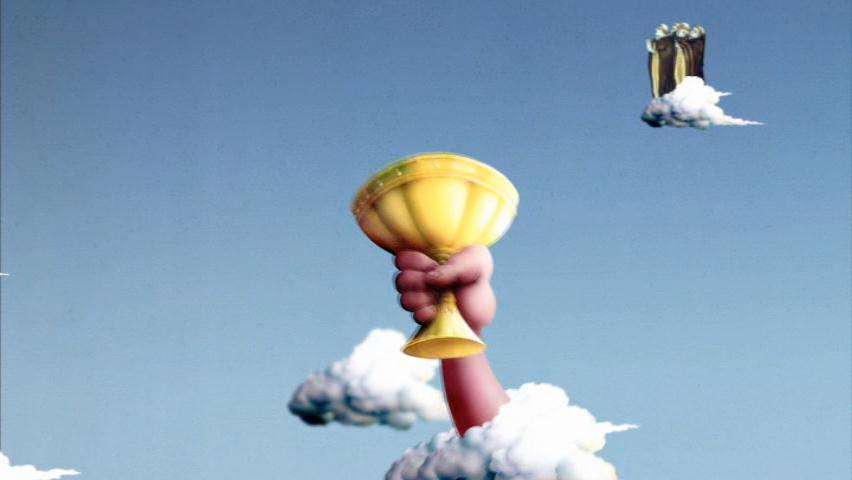
\includegraphics[width=0.8\textwidth]{grail.jpg}
  \caption[Voorbeeld figuur.]{\label{fig:grail}Voorbeeld van invoegen van een figuur. Zorg altijd voor een uitgebreid bijschrift dat de figuur volledig beschrijft zonder in de tekst te moeten gaan zoeken. Vergeet ook je bronvermelding niet!}
\end{figure}

\begin{listing}
  \begin{minted}{python}
    import pandas as pd
    import seaborn as sns

    penguins = sns.load_dataset('penguins')
    sns.relplot(data=penguins, x="flipper_length_mm", y="bill_length_mm", hue="species")
  \end{minted}
  \caption[Voorbeeld codefragment]{Voorbeeld van het invoegen van een codefragment.}
\end{listing}

\lipsum[7-20]

\begin{table}
  \centering
  \begin{tabular}{lcr}
    \toprule
    \textbf{Kolom 1} & \textbf{Kolom 2} & \textbf{Kolom 3} \\
    $\alpha$         & $\beta$          & $\gamma$         \\
    \midrule
    A                & 10.230           & a                \\
    B                & 45.678           & b                \\
    C                & 99.987           & c                \\
    \bottomrule
  \end{tabular}
  \caption[Voorbeeld tabel]{\label{tab:example}Voorbeeld van een tabel.}
\end{table}


%%=============================================================================
%% Methodologie
%%=============================================================================

\chapter{\IfLanguageName{dutch}{Methodologie}{Methodology}}%
\label{ch:methodologie}

%% TODO: In dit hoofstuk geef je een korte toelichting over hoe je te werk bent
%% gegaan. Verdeel je onderzoek in grote fasen, en licht in elke fase toe wat
%% de doelstelling was, welke deliverables daar uit gekomen zijn, en welke
%% onderzoeksmethoden je daarbij toegepast hebt. Verantwoord waarom je
%% op deze manier te werk gegaan bent.
%% 
%% Voorbeelden van zulke fasen zijn: literatuurstudie, opstellen van een
%% requirements-analyse, opstellen long-list (bij vergelijkende studie),
%% selectie van geschikte tools (bij vergelijkende studie, "short-list"),
%% opzetten testopstelling/PoC, uitvoeren testen en verzamelen
%% van resultaten, analyse van resultaten, ...
%%
%% !!!!! LET OP !!!!!
%%
%% Het is uitdrukkelijk NIET de bedoeling dat je het grootste deel van de corpus
%% van je graduaatsproef in dit hoofstuk verwerkt! Dit hoofdstuk is eerder een
%% kort overzicht van je plan van aanpak.
%%
%% Maak voor elke fase (behalve het literatuuronderzoek) een NIEUW HOOFDSTUK aan
%% en geef het een gepaste titel.

\lipsum[21-25]



% Voeg hier je eigen hoofdstukken toe die de ``corpus'' van je graduaatsproef
% vormen. De structuur en titels hangen af van je eigen onderzoek. Je kan bv.
% elke fase in je onderzoek in een apart hoofdstuk bespreken.

%\input{...}
%\input{...}
%...

%%=============================================================================
%% Conclusie
%%=============================================================================

\chapter{Conclusie}%
\label{ch:conclusie}

Het doel van deze graduaatsproef was het ontwikkelen van een mobiele applicatie die gebruikers met chronische gezondheidsproblemen ondersteunt bij het registreren van menstruatiecycli, voeding, pijnklachten en medicatie-inname. Deze onderzoeksvraag werd beantwoord door middel van een combinatie van literatuuronderzoek, analyse van bestaande applicaties en het ontwikkelen van een werkend prototype met Flutter.

Uit het onderzoek bleek dat er een duidelijke nood bestaat aan centralisatie van gezondheidstracking. Bestaande apps zijn vaak gefragmenteerd en beperken zich tot één specifiek domein, wat het voor gebruikers moeilijk maakt om verbanden te leggen tussen verschillende gezondheidsfactoren. De Unda Health Tracker biedt hierop een antwoord door meerdere trackers in één overzichtelijke app te combineren.

De keuze voor Flutter als ontwikkeltool heeft zich in de praktijk bewezen als een geschikte keuze. Dankzij de declaratieve structuur, het gebruik van herbruikbare widgets en de mogelijkheid om performant te compileren naar native code, kon een applicatie gebouwd worden die intuïtief aanvoelt en op meerdere platformen draait.

De ontwikkelde app maakt het mogelijk voor gebruikers om snel en eenvoudig hun gezondheidsgegevens in te voeren, te visualiseren en eventueel te delen met zorgverleners. Deze functionaliteit draagt bij aan een beter zelfmanagement van chronische klachten, en biedt ook voor artsen een meer gestructureerde en objectieve kijk op subjectieve symptomen zoals pijn of vermoeidheid.

Hoewel het prototype een solide basis vormt, zijn er nog verschillende aspecten die verder kunnen worden uitgewerkt. Zo kan de app uitgebreid worden met gepersonaliseerde meldingen, synchronisatie met wearables, en integratie van AI om automatisch patronen te herkennen. Verder onderzoek zou zich ook kunnen richten op gebruikersonderzoek met grotere testgroepen en langdurige evaluatie in een klinische context.

Samengevat toont deze graduaatsproef aan dat een centrale, gebruiksvriendelijke mobiele applicatie zoals Unda effectief kan bijdragen aan het verbeteren van gezondheidstracking voor mensen met chronische aandoeningen. Het biedt een meerwaarde voor zowel gebruikers als zorgverleners, en vormt een veelbelovende basis voor verdere ontwikkeling binnen het domein van mHealth.




%---------- Bijlagen -----------------------------------------------------------

\appendix

\chapter{Onderzoeksvoorstel}

Het onderwerp van deze graduaatsproef is gebaseerd op een onderzoeksvoorstel dat vooraf werd beoordeeld door de promotor. Dat voorstel is opgenomen in deze bijlage.

%% TODO: 
%\section*{Samenvatting}

% Kopieer en plak hier de samenvatting (abstract) van je onderzoeksvoorstel.

% Verwijzing naar het bestand met de inhoud van het onderzoeksvoorstel
%---------- Inleiding ---------------------------------------------------------

% TODO: Is dit voorstel gebaseerd op een paper van Research Methods die je
% vorig jaar hebt ingediend? Heb je daarbij eventueel samengewerkt met een
% andere student?
% Zo ja, haal dan de tekst hieronder uit commentaar en pas aan.

%\paragraph{Opmerking}

% Dit voorstel is gebaseerd op het onderzoeksvoorstel dat werd geschreven in het
% kader van het vak Research Methods dat ik (vorig/dit) academiejaar heb
% uitgewerkt (met medesturent VOORNAAM NAAM als mede-auteur).
% 

\section{Inleiding}%
\label{sec:inleiding}

Mijn graduaatsproef richt zich op de ontwikkeling van een mobiele applicatie die gebruikers ondersteunt bij het bijhouden van menstruatiecycli, eet- en drinkgewoonten, pijnervaringen en medicatie-inname. Dit project komt voort uit een persoonlijke behoefte aan een geïntegreerd platform waarin al deze gegevens eenvoudig en overzichtelijk kunnen worden opgeslagen. De doelgroep bestaat uit personen met chronische aandoeningen of hormonale schommelingen die medische gegevens moeten bijhouden, evenals gezondheidsbewuste gebruikers die hun levensstijl willen monitoren.

De centrale probleemstelling luidt: "Hoe kan een mobiele applicatie bijdragen aan een efficiënte en overzichtelijke registratie van menstruatiecycli, voeding, pijnklachten en medicatie-inname?" Momenteel moeten gebruikers vaak meerdere applicaties of fysieke notities gebruiken, wat leidt tot een gefragmenteerd overzicht en mogelijke dataverlies. De onderzoeksdoelstelling is daarom het ontwikkelen van een gebruiksvriendelijke applicatie die deze gegevens op een logische en samenhangende manier samenbrengt. Dit onderzoek zal resulteren in een functionele mobiele applicatie die de registratie en visualisatie van deze gegevens optimaliseert.

%---------- Stand van zaken ---------------------------------------------------

\section{Literatuurstudie}%
\label{sec:literatuurstudie}
Het bijhouden van gezondheidsgegevens is een essentieel onderdeel van zelfzorg en medische opvolging. Menstruatietracking-apps kunnen helpen bij het identificeren van patronen in de cyclus en hormonale schommelingen. Voedingsdagboeken kunnen bijdragen aan een gezondere levensstijl en betere medische diagnoses. Pijnregistratie wordt vaak toegepast bij chronische aandoeningen, waarbij een gedetailleerde logboekfunctie nuttig kan zijn voor medische professionals. Ten slotte zijn medicatieherinneringen zeer handig voor zowel anticonceptie als andere belangrijke medicatie. 

Hoewel er al verschillende apps bestaan die zich focussen op afzonderlijke aspecten van gezondheidstracking, ontbreekt een geïntegreerde oplossing die al deze functies combineert. Dit onderzoek richt zich op de ontwikkeling van een applicatie die deze gegevens op een gecentraliseerde manier beheert, waardoor gebruikers een beter inzicht krijgen in hun gezondheid.

%---------- Methodologie ------------------------------------------------------
\section{Methodologie}%
\label{sec:methodologie}
Ik ben van plan om Flutter te gebruiken om mijn cross-platform mobile applicatie te maken.
%---------- Verwachte resultaten ----------------------------------------------
\section{Verwacht resultaat, conclusie}%
\label{sec:verwachte_resultaten}

Het verwachte resultaat van deze graduaatsproef is een functionele mobiele applicatie die menstruatiecycli, voeding, pijnervaringen en medicatie-inname overzichtelijk bijhoudt. Door deze geïntegreerde aanpak krijgen gebruikers een volledig beeld van hun gezondheid en kunnen ze beter geïnformeerde beslissingen nemen.

De meerwaarde van dit onderzoek ligt in de verbetering van zelfmonitoring en medische opvolging. Gebruikers zullen in staat zijn om eenvoudig en gestructureerd gegevens te verzamelen, wat hen helpt bij gesprekken met zorgverleners en het identificeren van gezondheidsproblemen. Daarnaast draagt deze applicatie bij aan de digitalisering en automatisering van gezondheidsregistratie, wat het gebruiksgemak en de efficiëntie verhoogt.

%%---------- Andere bijlagen --------------------------------------------------
% TODO: Voeg hier eventuele andere bijlagen toe. Bv. als je deze BP voor de
% tweede keer indient, een overzicht van de verbeteringen t.o.v. het origineel.
%\input{...}

%%---------- Backmatter, referentielijst ---------------------------------------

\backmatter{}

\setlength\bibitemsep{2pt} %% Add Some space between the bibliograpy entries
\printbibliography[heading=bibintoc]

\end{document}
